\documentclass[12pt,letterpaper]{article}
\usepackage{graphicx,textcomp}
\usepackage{natbib}
\usepackage{setspace}
\usepackage{fullpage}
\usepackage{color}
\usepackage[reqno]{amsmath}
\usepackage{amsthm}
\usepackage{fancyvrb}
\usepackage{amssymb,enumerate}
\usepackage[all]{xy}
\usepackage{endnotes}
\usepackage{lscape}
\newtheorem{com}{Comment}
\usepackage{float}
\usepackage{hyperref}
\newtheorem{lem} {Lemma}
\newtheorem{prop}{Proposition}
\newtheorem{thm}{Theorem}
\newtheorem{defn}{Definition}
\newtheorem{cor}{Corollary}
\newtheorem{obs}{Observation}
\usepackage[compact]{titlesec}
\usepackage{dcolumn}
\usepackage{tikz}
\usetikzlibrary{arrows}
\usepackage{multirow}
\usepackage{xcolor}
\usepackage{fancyvrb}
\newcolumntype{.}{D{.}{.}{-1}}
\newcolumntype{d}[1]{D{.}{.}{#1}}
\definecolor{light-gray}{gray}{0.65}
\usepackage{url}
\usepackage{listings}
\usepackage{color}
\usepackage{etoolbox}
\makeatletter
\preto{\@verbatim}{\topsep=0pt \partopsep=0pt }
\makeatother
\usepackage{placeins}



\definecolor{codegreen}{rgb}{0,0.6,0}
\definecolor{codegray}{rgb}{0.5,0.5,0.5}
\definecolor{codepurple}{rgb}{0.58,0,0.82}
\definecolor{backcolour}{rgb}{0.95,0.95,0.92}

\lstdefinestyle{mystyle}{
	backgroundcolor=\color{backcolour},   
	commentstyle=\color{codegreen},
	keywordstyle=\color{magenta},
	numberstyle=\tiny\color{codegray},
	stringstyle=\color{codepurple},
	basicstyle=\footnotesize,
	breakatwhitespace=false,         
	breaklines=true,                 
	captionpos=b,                    
	keepspaces=true,                 
	numbers=left,                    
	numbersep=5pt,                  
	showspaces=false,                
	showstringspaces=false,
	showtabs=false,                  
	tabsize=2
}
\lstset{style=mystyle}
\newcommand{\Sref}[1]{Section~\ref{#1}}
\newtheorem{hyp}{Hypothesis}



\title{Problem Set 4}
\date{Due: November 27, 2025}
\author{Ellen Beattie}


\begin{document}
	\maketitle



\section*{Question 1: Economics}
\vspace{.25cm}
\noindent 	
Loading \texttt{prestige} dataset in the \texttt{car} library
\lstinputlisting[language=R, firstline=27, lastline=30]{PS04_EB.R}
\vspace{.25cm}

\noindent We would like to study whether individuals with higher levels of income have more prestigious jobs. Moreover, we would like to study whether professionals have more prestigious jobs than blue and white collar workers.

\vspace*{2cm}
\begin{enumerate}
	
	\item [(a)]
	Create a new variable \texttt{professional} by recoding the variable \texttt{type} so that professionals are coded as $1$, and blue and white collar workers are coded as $0$ (Hint: \texttt{ifelse}).
	
	\lstinputlisting[language=R, firstline=37, lastline=39]{PS04_EB.R}
	\vspace{0.25cm}
	
	\newpage
	\item [(b)]
	Run a linear model with \texttt{prestige} as an outcome and \texttt{income}, \texttt{professional}, and the interaction of the two as predictors (Note: this is a continuous $\times$ dummy interaction.)
	
	\lstinputlisting[language=R, firstline=42, lastline=47]{PS04_EB.R}
	
	% Table created by stargazer v.5.2.3 by Marek Hlavac, Social Policy Institute. E-mail: marek.hlavac at gmail.com
	% Date and time: Thu, Nov 27, 2025 - 10:04:07
	\begin{table}[!htbp] \centering 
		\caption{Impact of Income level and being a Professional on Job Prestige} 
		\label{} 
		\begin{tabular}{@{\extracolsep{5pt}}lc} 
			\\[-1.8ex]\hline 
			\hline \\[-1.8ex] 
			& \multicolumn{1}{c}{\textit{Dependent variable:}} \\ 
			\cline{2-2} 
			\\[-1.8ex] &  Prestige \\ 
			\hline \\[-1.8ex] 
			Income & 0.003$^{***}$ \\ 
			& (0.0005) \\ 
			& \\ 
			Professional & 37.781$^{***}$ \\ 
			& (4.248) \\ 
			& \\ 
			Income*Professional & $-$0.002$^{***}$ \\ 
			& (0.001) \\ 
			& \\ 
			Constant & 21.142$^{***}$ \\ 
			& (2.804) \\ 
			& \\ 
			\hline \\[-1.8ex] 
			Observations & 98 \\ 
			R$^{2}$ & 0.787 \\ 
			Adjusted R$^{2}$ & 0.780 \\ 
			Residual Std. Error & 8.012 (df = 94) \\ 
			F Statistic & 115.878$^{***}$ (df = 3; 94) \\ 
			\hline 
			\hline \\[-1.8ex] 
			\textit{Note:}  & \multicolumn{1}{r}{$^{*}$p$<$0.1; $^{**}$p$<$0.05; $^{***}$p$<$0.01} \\ 
		\end{tabular} 
	\end{table} 
	\FloatBarrier
	There is a positive and statistically reliable relationship between income, being a professional and income*professional interaction on prestige. The model explains 78.7\% of the total variation in prestige.  
	\newpage
	\lstinputlisting[language=R, firstline=49, lastline=64]{PS04_EB.R}
	\begin{figure}[!htbp]\centering
	\caption{\footnotesize Plot of Prestige, Income and Professional}
	\label{fig:plot_4}
	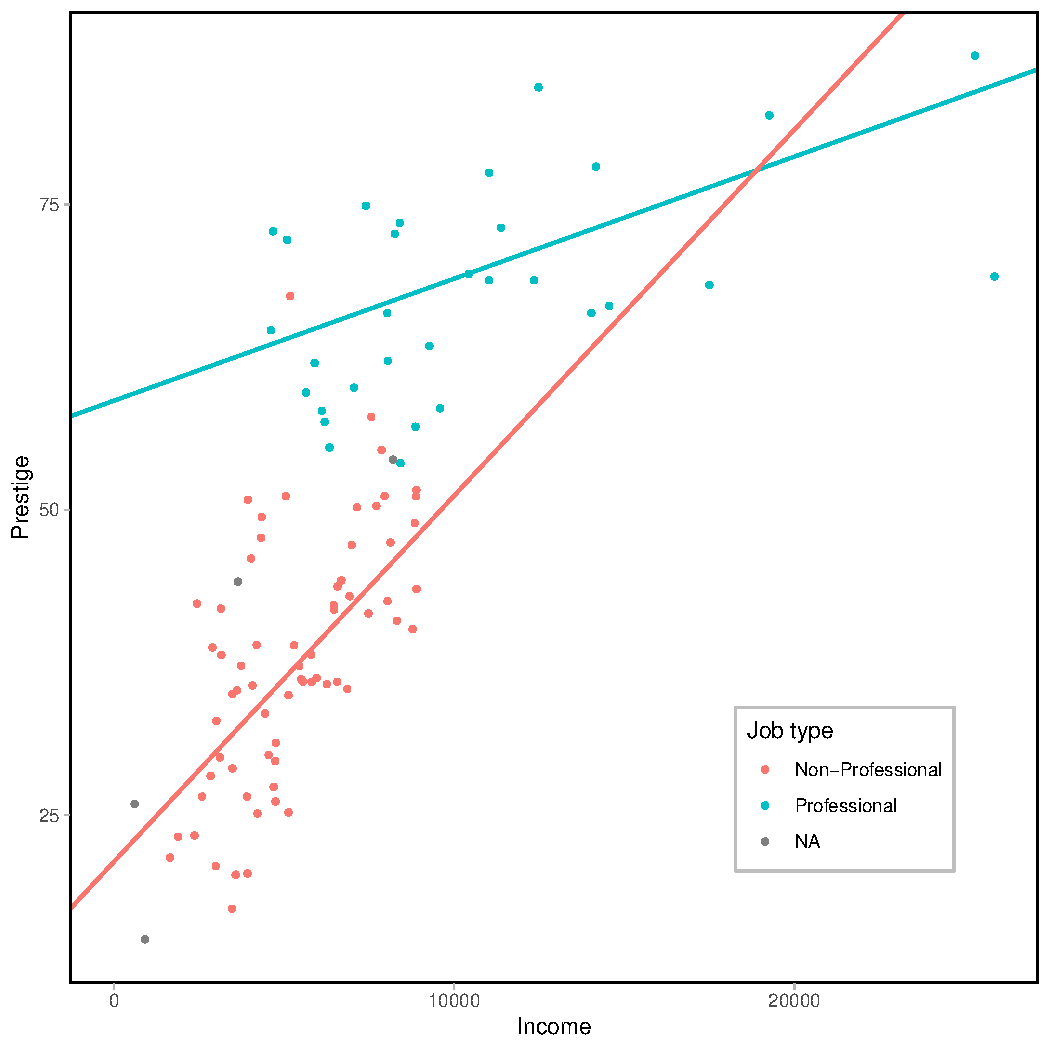
\includegraphics[width=.7\textwidth]{PS04_reg1plot.pdf}
	\end{figure}
	\FloatBarrier
	
	\newpage
	\vspace{0.5cm}
	\item [(c)]
	Write the prediction equation based on the result.
	\begin{equation}
		\hat{y} = \hat{\beta_0} + \hat{\beta_1}\texttt{income} + \hat{\beta_2}\texttt{professional} - \hat{\beta_3}(\texttt{income}\times \texttt{professional})
	\end{equation}
	\begin{equation}
		\widehat{\text{prestige}} = 21.142 + 0.003\times\text{income} + 37.781\times\text{professional} - 0.002\times(\text{income}\times \text{professional})
	\end{equation}
	
	\vspace*{1cm}
	\item [(d)]
	Interpret the coefficient for \texttt{income}. \\
	
	The income coefficient $\beta_1 = 0.003$ represents the expected impact of a one unit increase in income for the non-professionals (reference group where non-professional = 0). That is,  a one unit increase in income is, on average, associated with a 0.003 increase in prestige for non-professionals. \\
	
	Due to the interaction term income*professional, the effect of income for professionals differs to non-professionals by $\beta_3$ units. For professionals, a one unit increase in income is associated with, on average, 0.001 increase in prestige ($\beta_1 + \beta_3 = 0.003-0.002$). 
	
	
	\vspace{2cm}
	\item [(e)]
	Interpret the coefficient for \texttt{professional}.\\
	
	The professional coefficient $\beta_2 = 37.781$ represents the expected difference in prestige level being professional (when prof = 1) and non-professionals (when prof = 0) when income is zero. Being a professional essentially increases the base level of job prestige from 21.142 (just $\beta_0$) to 58.923 ($\beta_0 + \beta_3$) at the intercept.  \\
	
 	Due to the inclusion of an interaction term income*gender, the expected difference between professionals and non-professional prestige is different depending on their income level (unlike the constant effect of a dummy in an additive model).  Therefore, this interpretation is restricted to when income is 0, and should not be mistaken for the overall effect of being a professional.  
	
	\newpage
	\item [(f)]
	What is the effect of a \$1,000 increase in income on prestige score for professional occupations? In other words, we are interested in the marginal effect of income when the variable \texttt{professional} takes the value of $1$. Calculate the change in $\hat{y}$ associated with a \$1,000 increase in income based on your answer for (c). \\
	
	For professionals ($\texttt{professional} = 1$), the prediction equation  is: 
	\begin{equation}
		\hat{y} = (\hat{\beta_0} + \hat{\beta_2}) +  (\hat{\beta_1} + \hat{\beta_3})\times \texttt{income} = 58.923 + 0.001 \times\text{income}
	\end{equation}

	Therefore to calculate the marginal effect of income ($ME_{income}$), determine change in prestige associated with a change in income. 
	\begin{equation}
		\text{Professional with \$0 income}: \quad \hat{y} = 58.923 + 0.001 \times 0 = 58.923
	\end{equation}
	\begin{equation}
		\text{Professional with \$1000 income}: \quad \hat{y} = 58.923 + 0.001 \times 1000 = 59.923
	\end{equation}
	\begin{equation}
		\text{Professional with \$2000 income}: \quad \hat{y} = 58.923 + 0.001 \times 2000 = 60.923
	\end{equation}
	\begin{equation}
		ME_{income} = \frac{\Delta\hat{y}}{\Delta\text{income}} = \frac{(59.923-58.923)}{1000-0} =\frac{1}{1000} = 0.001 = (\beta_1 + \beta_3)
	\end{equation}
	
	Increasing income by \$1000 for professionals increases their prestige score by 0.001 (i.e. the $\beta_1 +\beta_3$). This marginal effect of income on professionals is constant, meaning the no matter the income level the effect of increasing income by \$1000 is the same. However, this marginal effect is only for professionals, and is different to the marginal effect of income on non-professionals which is also constant but equals $\beta_1$. 
	
	
	\vspace{0.75cm}
	
	
	\item [(g)]
	What is the effect of changing one's occupations from non-professional to professional when her income is \$6,000? We are interested in the marginal effect of professional jobs when the variable \texttt{income} takes the value of $6,000$. Calculate the change in $\hat{y}$ based on your answer for (c).
	
	\begin{equation}
		\text{Professional with \$6000 income}: \quad \hat{y} = 58.923 + 0.001 \times 0 = 64.923
	\end{equation}
	\begin{equation}
		\text{Non-Professional with \$6000 income}: \quad \hat{y} = 21.142 + 0.003 \times 6000 = 39.142
	\end{equation}
	\begin{equation}
		ME_{professional|income=\$6000} = \frac{\Delta\hat{y}}{\Delta\text{professional}} = \frac{(64.923-38.141)}{1-0} = 25.781
	\end{equation}
	The marginal effect of professional jobs when income is \$6000 is 25.781. 
	However, at different income levels the marginal effect of professional is different (e.g. at \$3000  $\Delta\hat{y}= 31.781$ and at \$9000 $\Delta\hat{y} = 19.731$).  
	$ ME_{\$9000} < ME_{\$6000} < ME_{\$3000}$, that is the effect of moving from non-professional to professional on prestige is different at different income levels.\\ As income increases the marginal effect is lower, intuitively the difference is largest at the intercept ($\beta_2$) and slowly decreases as income increases, with every unit increase of income having a bigger impact on non-professionals ($\beta_1 = 0.003$) than professionals($\beta_1 + \beta_3 = 0.001$).  
	
	
\end{enumerate}

\newpage

\section*{Question 2: Political Science}
\vspace{.25cm}
\noindent 	Researchers are interested in learning the effect of all of those yard signs on voting preferences.\footnote{Donald P. Green, Jonathan	S. Krasno, Alexander Coppock, Benjamin D. Farrer,	Brandon Lenoir, Joshua N. Zingher. 2016. ``The effects of lawn signs on vote outcomes: Results from four randomized field experiments.'' Electoral Studies 41: 143-150. } Working with a campaign in Fairfax County, Virginia, 131 precincts were randomly divided into a treatment and control group. In 30 precincts, signs were posted around the precinct that read, ``For Sale: Terry McAuliffe. Don't Sellout Virgina on November 5.'' \\

Below is the result of a regression with two variables and a constant.  The dependent variable is the proportion of the vote that went to McAuliff's opponent Ken Cuccinelli. The first variable indicates whether a precinct was randomly assigned to have the sign against McAuliffe posted. The second variable indicates
a precinct that was adjacent to a precinct in the treatment group (since people in those precincts might be exposed to the signs).  \\

\vspace{.5cm}
\begin{table}[!htbp]
	\centering 
	\textbf{Impact of lawn signs on vote share}\\
	\begin{tabular}{@{\extracolsep{5pt}}lccc} 
		\\[-1.8ex] 
		\hline \\[-1.8ex]
		Precinct assigned lawn signs  (n=30)  & 0.042\\
		& (0.016) \\
		Precinct adjacent to lawn signs (n=76) & 0.042 \\
		&  (0.013) \\
		Constant  & 0.302\\
		& (0.011)
		\\
		\hline \\
	\end{tabular}\\
	\footnotesize{\textit{Notes:} $R^2$=0.094, N=131}
\end{table}

	\begin{equation*}
		\text{Regression Line}: Y_i = \beta_0 + \beta_1 x_{1i} + \beta_2 x_{2i} + \epsilon_i 
	\end{equation*}
	where $x_1$ = Precinct assigned lawn signs and $x_2$ = Precinct adjacent to lawn signs
	
	\newpage
\begin{enumerate}
	\item [(a)] Use the results from a linear regression to determine whether having these yard signs in a precinct affects vote share (e.g., conduct a hypothesis test with $\alpha = .05$). 
	\vspace{0.5cm}
	
	 We want to determine if having yard signs in a precinct affects vote share i.e. if there is a significant effect of $\beta_1$ in the model. So, using proof by contradiction we set up the null hypothesis that there is no effect of yard signs in a precinct on voteshare (i.e. the regression coefficient is 0)
	We then compute a test statistic using the coefficient and its standard error to determine the p-value with degrees of freedom  $df = (n - k - 1) = (131 - 2 - 1) = 128$ where k is the number of predictors in the multivariate model. 
	
	\begin{equation*}
	H_0: \beta_1 = 0, \quad H_1: \beta_1 \ne 0
	\end{equation*}
	\begin{equation*}
	\text{Test Statistic}; t = \frac{\hat{\beta_1}}{se_{\hat{\beta_1}}} = \frac{0.042}{0.016} = 2.625
	\end{equation*}

	\lstinputlisting[language=R, firstline=68, lastline=72]{PS04_EB.R}
	\begin{verbatim}
		[1] 2.625
		[1] 0.00972002
	\end{verbatim}
	
	We determine that the p-value is below the significance level threshold $p = 0.009 < 0.05 = \alpha$. Therefore, we find sufficient evidence to reject the null hypothesis that having yard signs in a precinct has no effect on voteshare.   
	

	
	
	\newpage
	\item [(b)]  Use the results to determine whether being
	next to precincts with these yard signs affects vote
	share (e.g., conduct a hypothesis test with $\alpha = .05$).
	\vspace{1cm}
	
	Using the same process as above, this time we are testing if having yard signs in an adjacent precinct affects vote share i.e. if there is a significant effect of $\beta_2$ in the model. So, using proof by contradiction we set up the null hypothesis that there is no effect of yard signs in an adjacent precinct on voteshare (i.e. the regression coefficient is 0). We again compute a test statistic to determine the p-value with degrees of freedom  $df = (n - k - 1) = (131 - 2 - 1) = 128$. 
	
	
		\begin{equation*}
		H_0: \beta_2 = 0, \quad H_1: \beta_2 \ne 0
	\end{equation*}
	\begin{equation*}
		\text{Test Statistic}; t = \frac{\hat{\beta_2}}{se_{\hat{\beta_2}}} = \frac{0.042}{0.013} = 3.231
	\end{equation*}
	\lstinputlisting[language=R, firstline=75, lastline=79]{PS04_EB.R}
	\begin{verbatim}
		[1] 3.230769
		[1] 0.00156946
	\end{verbatim}

	
	We determine that the p-value is below the significance level threshold $p = 0.001 < 0.05 = \alpha$. Therefore, we find sufficient evidence to reject the null hypothesis that having yard signs in an adjacent precinct has no effect on voteshare. 
	
	\vspace{2cm}
	\item [(c)] Interpret the coefficient for the constant term substantively. \\
	
	 McAuliff's opponent Ken Cuccinelli recieved 30.2\% of the vote in control group precincts that had no posted lawn signs or were not adjacent to any precincts with posted lawn signs. This acts as a baseline level that the impact of treatments is compared to. 
 
	\vspace{2cm}
	\newpage
	\item [(d)] Evaluate the model fit for this regression.  What does this	tell us about the importance of yard signs versus other factors that are not modeled? \\
	
	
	To evaluate the model fit for the regression we can conduct a global F-test that determines if the regression model is useful in explaining the outcome variation. It essentially tests the significance of all the predictor coefficients (full model) against a null model without the predictors (reduced model)
		\begin{equation*}
		\text{Full Model}: Y_i = \beta_0 + \beta_1 x_{1i} + \beta_2 x_{2i} + \epsilon_i \quad \text{vs}\quad\text{Reduced Model}: Y_i = \beta_0 + \epsilon_i 
	\end{equation*}
	Therefore the null hypothesis is that all variable predictors equal zero.
	\begin{equation*}
		H_0: \beta_1 = \beta_2 = 0 \quad \text{vs}\quad H_1: \text{At least one }\beta_j \ne 0
	\end{equation*}
	\begin{equation*}
		\text{F Statistic}; F = \frac{R^2_k /k}{(1-R^2_k)/(n-k-1)} = \frac{0.047}{0.00707} = 6.640
	\end{equation*}
	where $R^2_k$ = sample multiple multiple correlation coefficient, k = number of predictor variables, n = number of observations in sample
	\begin{equation*}
	 	F_{2,128} = 6.640, p = 0.0018
	\end{equation*}
	
	\lstinputlisting[language=R, firstline=83, lastline=87]{PS04_EB.R}
	\begin{verbatim}
		[1] 6.640177
		[1] 0.001803868
	\end{verbatim}
	Since p-value is very small we can reject the null hypothesis that all predictor coefficients are zero and accept that at least one of the model predictors are useful in explaining voteshare. 
	
\end{enumerate}  

	

\end{document}
